\documentclass[12pt,oneside,english]{article}

\usepackage[T1]{fontenc}
\usepackage[latin1]{inputenc}
\usepackage{geometry}
\geometry{verbose,letterpaper,tmargin=1in,bmargin=1in,lmargin=1in,rmargin=1in}
\usepackage{textcomp}
\usepackage{babel}
\setcounter{secnumdepth}{0}
\usepackage{graphicx}
\usepackage{float}
\floatstyle{boxed}
\restylefloat{figure}
\usepackage{longtable}
\usepackage{url}

\newcommand{\BibTeX}{{\sc Bib}\TeX}


\begin{document}
%\sffamily

        \title{in-situ impedance and morphology of self-assembling gold nanoislands}

	\author{John Donovan, Dr. Chuhee Kwon\\
	University of California, Long Beach, CA\\
	{\small donovan.csulb@gmail.com ckwon@csulb.edu}}
	
        \date{\today}

	\maketitle

	\tableofcontents
	

        \section{Introduction}

[ ancient intro junk until page 3 -- i'll fix this up in the next week ]

	\begin{figure}
	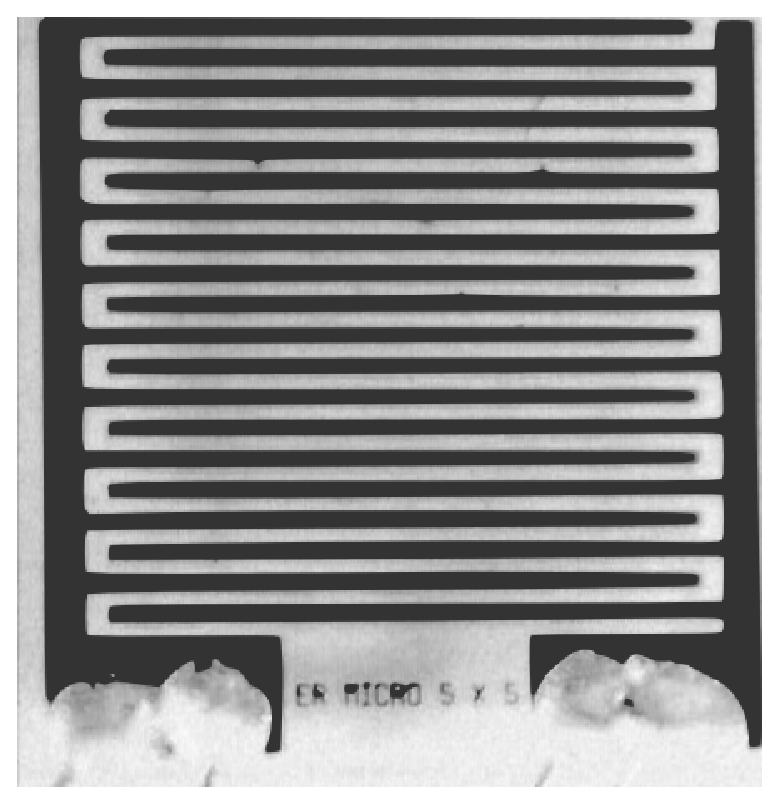
\includegraphics[width=60mm]{images/IDE.eps} \label{f:IDE}
	\caption{The self-assembling gold monolayers are deposited on a gold inter-digitized electrode (IDE).}
	\end{figure}
	
	Gold nanoislands  are formed by annealing a substrate -- on which gold has been uniformly deposited -- to produce islands within a predictable range of size and shape.
	
	This research attempts to characterizes the reproducibility of gold nano-island morphology using the polymer-assisted deposition and self-assembly method.
	
	Prior research suggests that the physical properties of gold nano-islands are sensitive to the method of depositing the gold, the number of layers, and variations in annealing temperature \cite{shon11}.

	[The LSPR absorption features of colloidal gold are shown by Kedem and Rubinstein (2011 acs) [add to bibtex, make sure it's original research]

 [there is more research to cite here -- lots of study of self-assembled islands from evaporative deposition by Van Duyne and his chain of relevant citations show properties vs. size et cetera, and I should find the proper method of citing other people's figures].  


	Gold nano-island formation through polymer-assisted self-assembly is also sensitive to the initial size of the colloidal gold used to form the self-assembling layers \\cite(reference), to the temperature profile during annealing, and to the length of time (in days) between creation and annealing (\cite{joshi}).

	[ more junk to clean up -- if I analyze how the polymer-deposited samples decay in air, it'll be done near the end of my research and be given a single paragraph and one figure ]
	
	This research quantifies the repeatiblity of gold nano-islands produced using the label-free(*) self-assembly method.

	[quote junk: I want these somewhere]
	
	\begin{quote}
	Plasmonic nanoparticles also act as transducers that convert small changes in the local refractive index into spectral shifts in the intense nanoparticle extinction and scattering spectra. 
	Most organic molecules have a higher refractive index than buffer solution; thus, when they bind to nanoparticles, the local refractive index increases, causing the extinction and scattering spectrum to redshift. 
	Molecular binding can be monitored in real time with high sensitivity by using simple and inexpensive transmission spectrometry, which measures extinction, the sum of absorption and scattering 3,8-10,41,42. 
	\cite{nature2008}
	\end{quote}

\begin{quote}
Thus, changes in the local environment - such as through the presence of an adsorbed species - should cause a shift in $\lambda_max$ .
\cite{willets2006}
\end{quote}

	\begin{figure}
		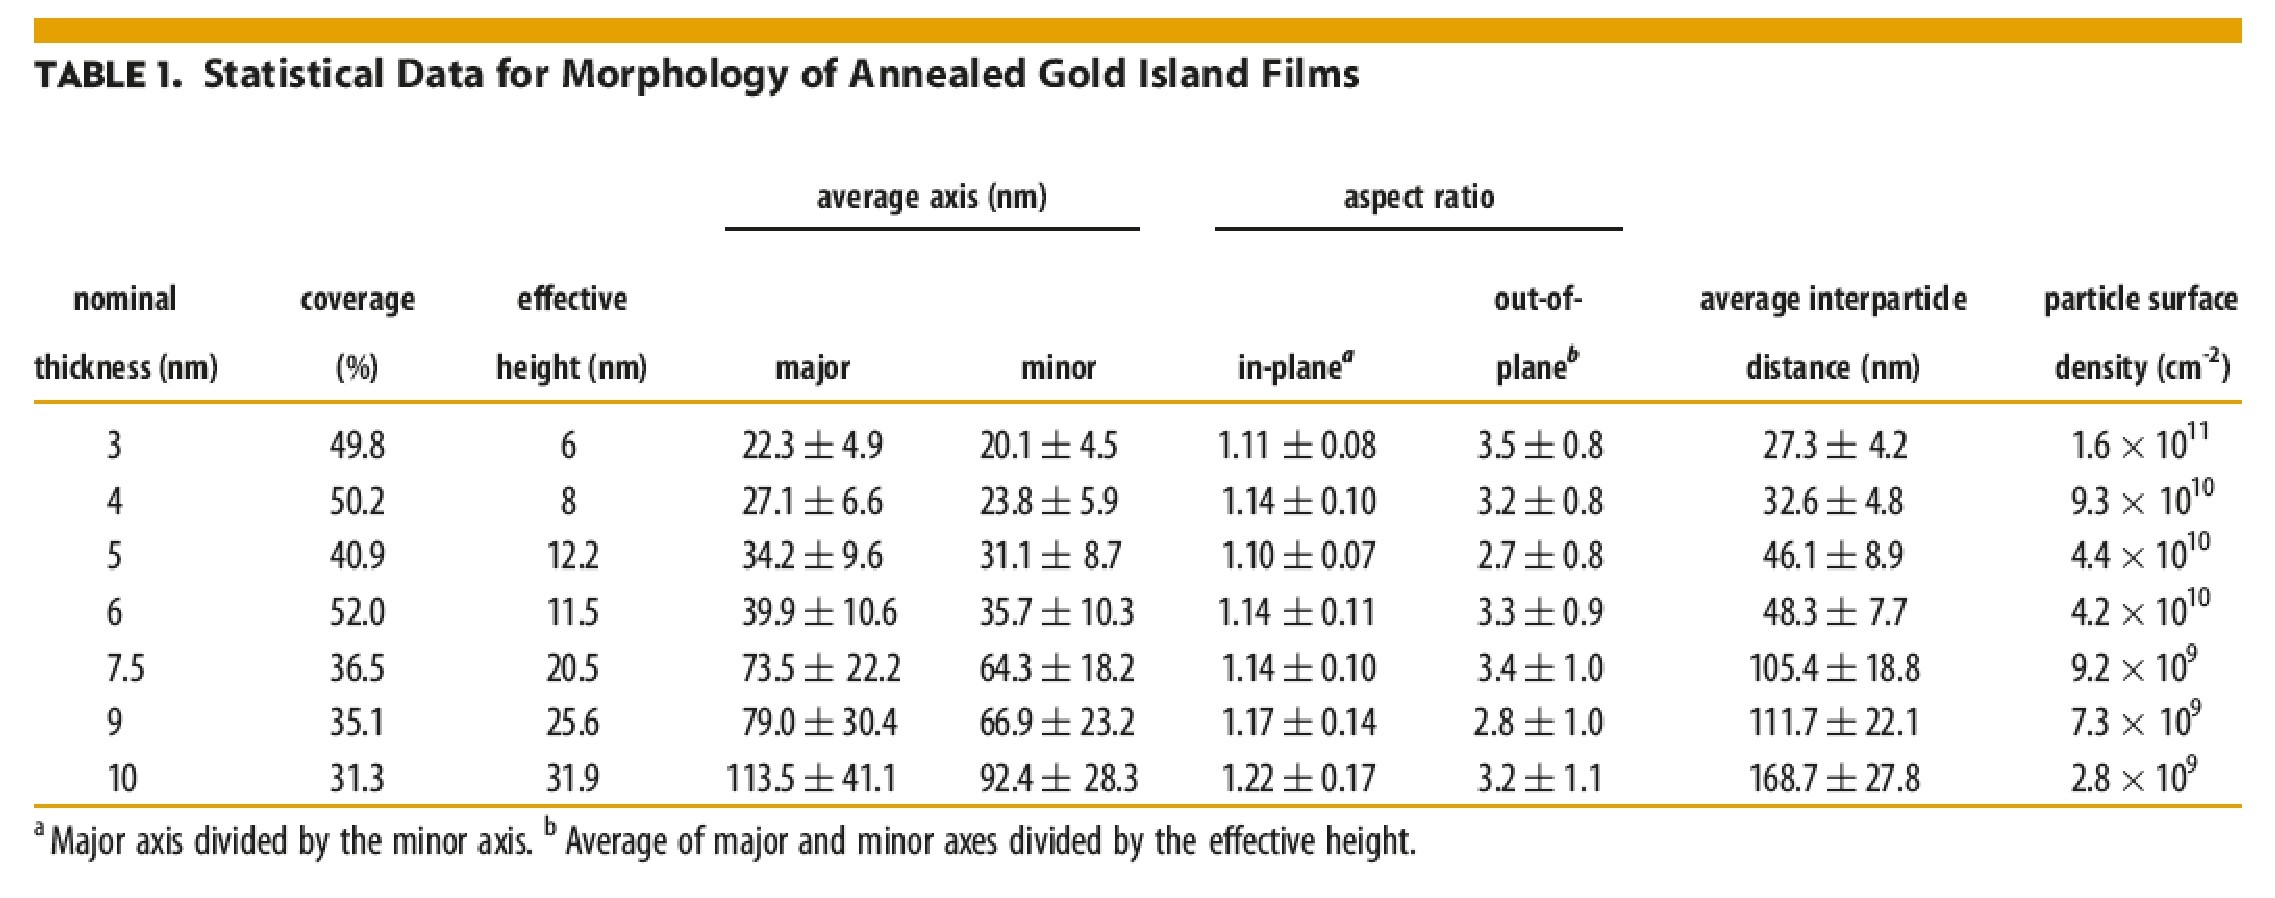
\includegraphics[width=120mm]{images/2011_Kedem_morphology.eps}
		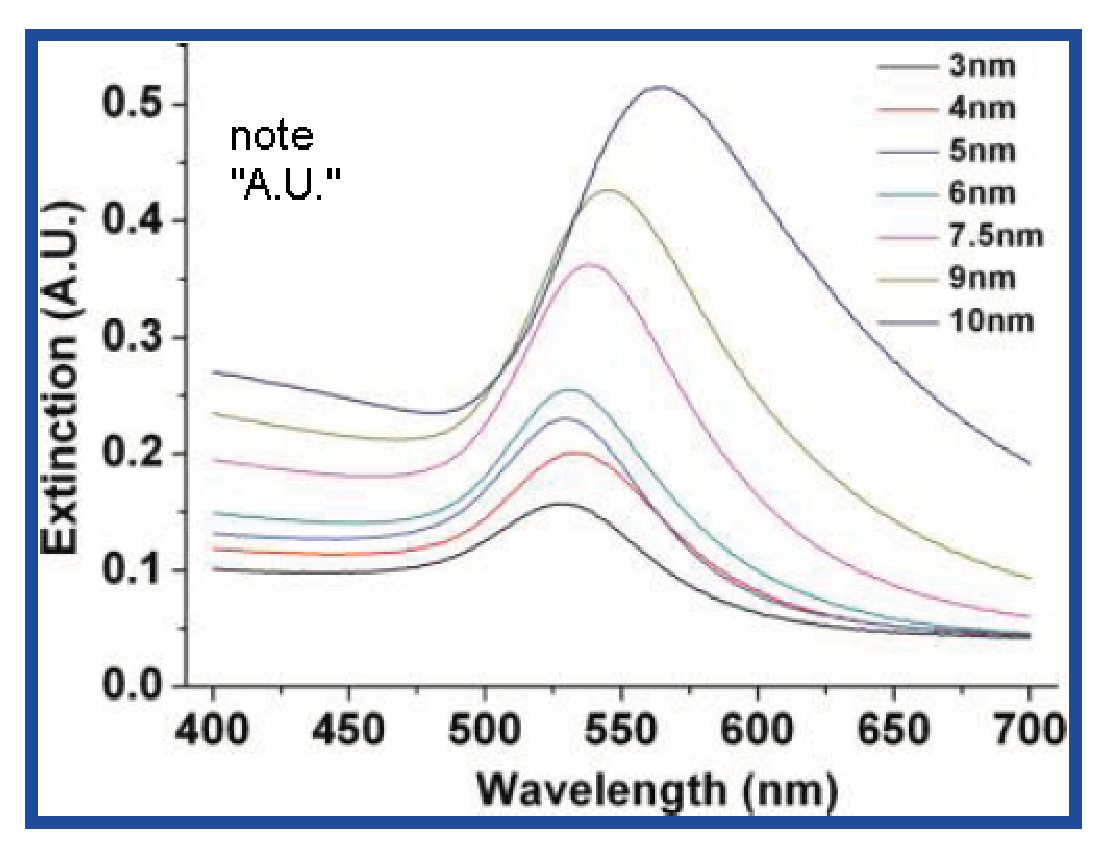
\includegraphics[width=50mm]{images/2011_Kedem_spectroscopy.eps}
		\caption{Two promenant figures should be a morphology characterization table and characteristic LSPR spectra with error bars if I can pull it off well-enough.}
	\end{figure}


	\subsection{The Chemistry of Self-Assembling Films}

	\emph{COMMENT: This section is based on discussion with YS Shon, and attribution should be made for these ideas.}
	
	Gold self-assembling films were produced from two sizes of gold particle.  
	The larger particles were Au$_{314}$, the smaller were Au$_{25}$.  
	These particles are coated in different organic ligands, which aid their solubility in ethanol (in the case of Au$_{314}$) and water (in the case of Au$_{25}$).    
	The ligands are terminated with a carboxy group (COOH) in ethanol and aqueous solutions; in the aqueous Au$_{25}$ solution, ligands may also be terminated with a positively charged carboxy group (COO-). 
	
	After the first gold layer is deposited the sample is dipped in an aqueous solution of poly(allyl-amine hydrochloride) (PAH).  
	The PAH bonds to the ligands and allows the next layer to assemble.  	
	The aqueous PAH molecules are terminated with amine groups (NH$_2$) and with positively charged amine groups (NH$_3^+$).  
	The relative occurrence of the NH$_3^+$ groups determine the pH of the solution.
	
	In the aqueous Au$_{25}$ solution, the PAH NH$_3^+$ group favorably bonds to the ligand COOH and COO- groups.
	The density of the single self-assembled gold layer therefore depends (non-linearly) on the pH of the PAH solution, with lower pH (higher ratio of NH$_3^+$ groups) resulting in higher packing density.
	The effect of pH on Au$_{25}$ layer density may be studied in this or another paper.
	
	In the ethanol Au$_{314}$ solution, there is an absence of ligand COO- groups.
	A more neutral pH of the PAH solution allows more bonds between NH$_2$ and COOH groups.
	
	\subsection{A model of gold density in Au$_{314}$ and Au$_{25}$ films}
	The difference in gold density between self-assembling Au$_{314}$ and Au$_{25}$ films can be visually observed.
	In previous unpublished study, an gold film formed from 8-layers of self-assembled Au$_{25}$ was equivalent in color to a Au$_{314}$ film of approximately 2-4 layers.
	The relationship between color and gold film thickness is a well-documented one, for films deposited by evaporation.
	If the color of a nano-island film is observed, the color may be misleading, as nano-island phonons depend not just on thickness, but also size and shape of the islands \cite{link99} (cite VanDuyne paper that shows islands up to $99{\mu}m$ diameter and their resulting LSPR absorption peaks).
	The size and shape of nano-islands depends on factors that include the initial size of the colloidal gold.
	
	To reach a first-order approximation of the relative gold density of Au$_{314}$ and Au$_{25}$ films, some assumptions must be made.
	First, the average length of the ligands are assumed to be fixed (we neglect that these ligands can easily stretch or shrink).
	Also, the effect of the pH in the PAH solution on packing density should be considered a second-order effect until demonstrated otherwise.	
	
	\begin{figure}
		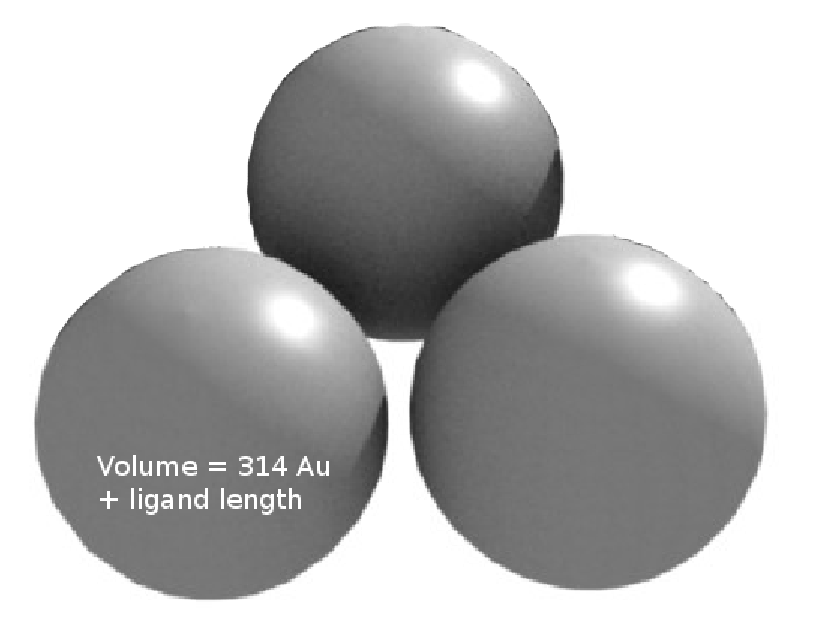
\includegraphics[width=60mm]{images/willitblend-big.eps}
		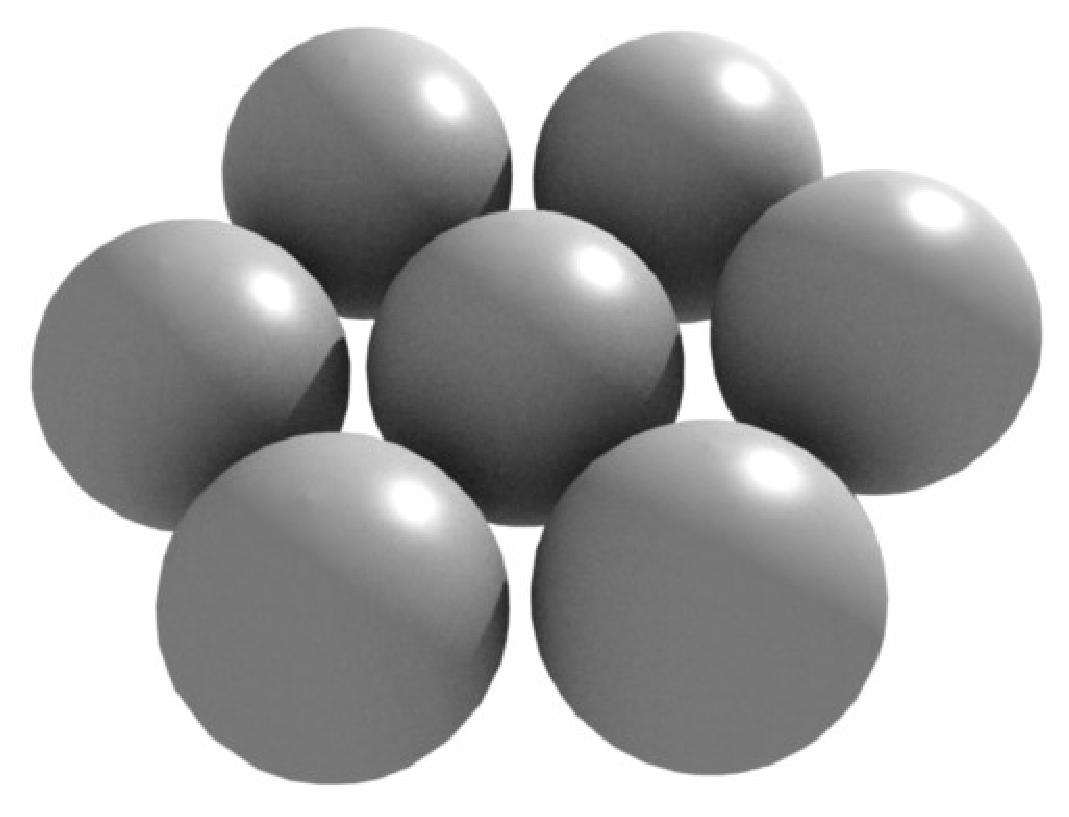
\includegraphics[width=50mm]{images/willitblend.eps}
		\caption{layered gold may be modeled as packed spheres whose packing density depends on radius (approximated) and amount of gold deposited per sphere (known).}
	\end{figure}
	[image in which the gold particles are modeled as packed spheres]	
	
	The approximate ligand length is 2${\mu}m$ for Au$_{314}$ and approximately 1${\mu}m$ for Au$_{25}$.
	The approximate size of the colloidal gold particles are 2.5${\mu}m$ for Au$_{314}$ and 1${\mu}m$ for Au$_{25}$.
	Making the assumption that these particles can be modeled as spheres of radius 3${\mu}m$ for Au$_{314}$ and 1.5${\mu}m$ for Au$_{25}$ leads to a relative density of 4 nanoparticles of Au$_{25}$ per nanoparticle of Au$_{314}$, which yields an approximate density of 100/314.
	
	At the first order, three times more layers of Au$_{25}$ should therefore be deposited to yield an equivalent gold mass to the Au$_{314}$ film.
	
	In real application, thermolysis of much more than 8 layers of a film will result in defects of significant density to affect the production of our nanoislands of interest.
	It is therefore better to use larger Au$_{314}$ particles instead of many layers of Au$_{25}$.


	\subsection{Size and Shape Distributions and Phonon Absorption Features}
	The uniformity of the size and shape is expected to correlate with the width of the absorption feature of the resulting sample.
	A wider distribution of sizes and shapes is expected to produce a broader absorption peak, while a narrower distribution of nanoisland sizes about the average size is expected to produce a sharper absorption feature.
	This relationship is predicted analytically because identical islands should absorb identically (neglecting second-order effects), producing a maximized peak.  
	Differences among the islands will create phonons that are offset by some amount from the peak wavelength, resulting in a lower and broader peak.

	Measurements of colloidal gold (Figure \ref{f:link99} \cite{link99}) show that peak depends on size and shape [lots of van duyne citations or citations to his original sources].
	
	\begin{figure}
		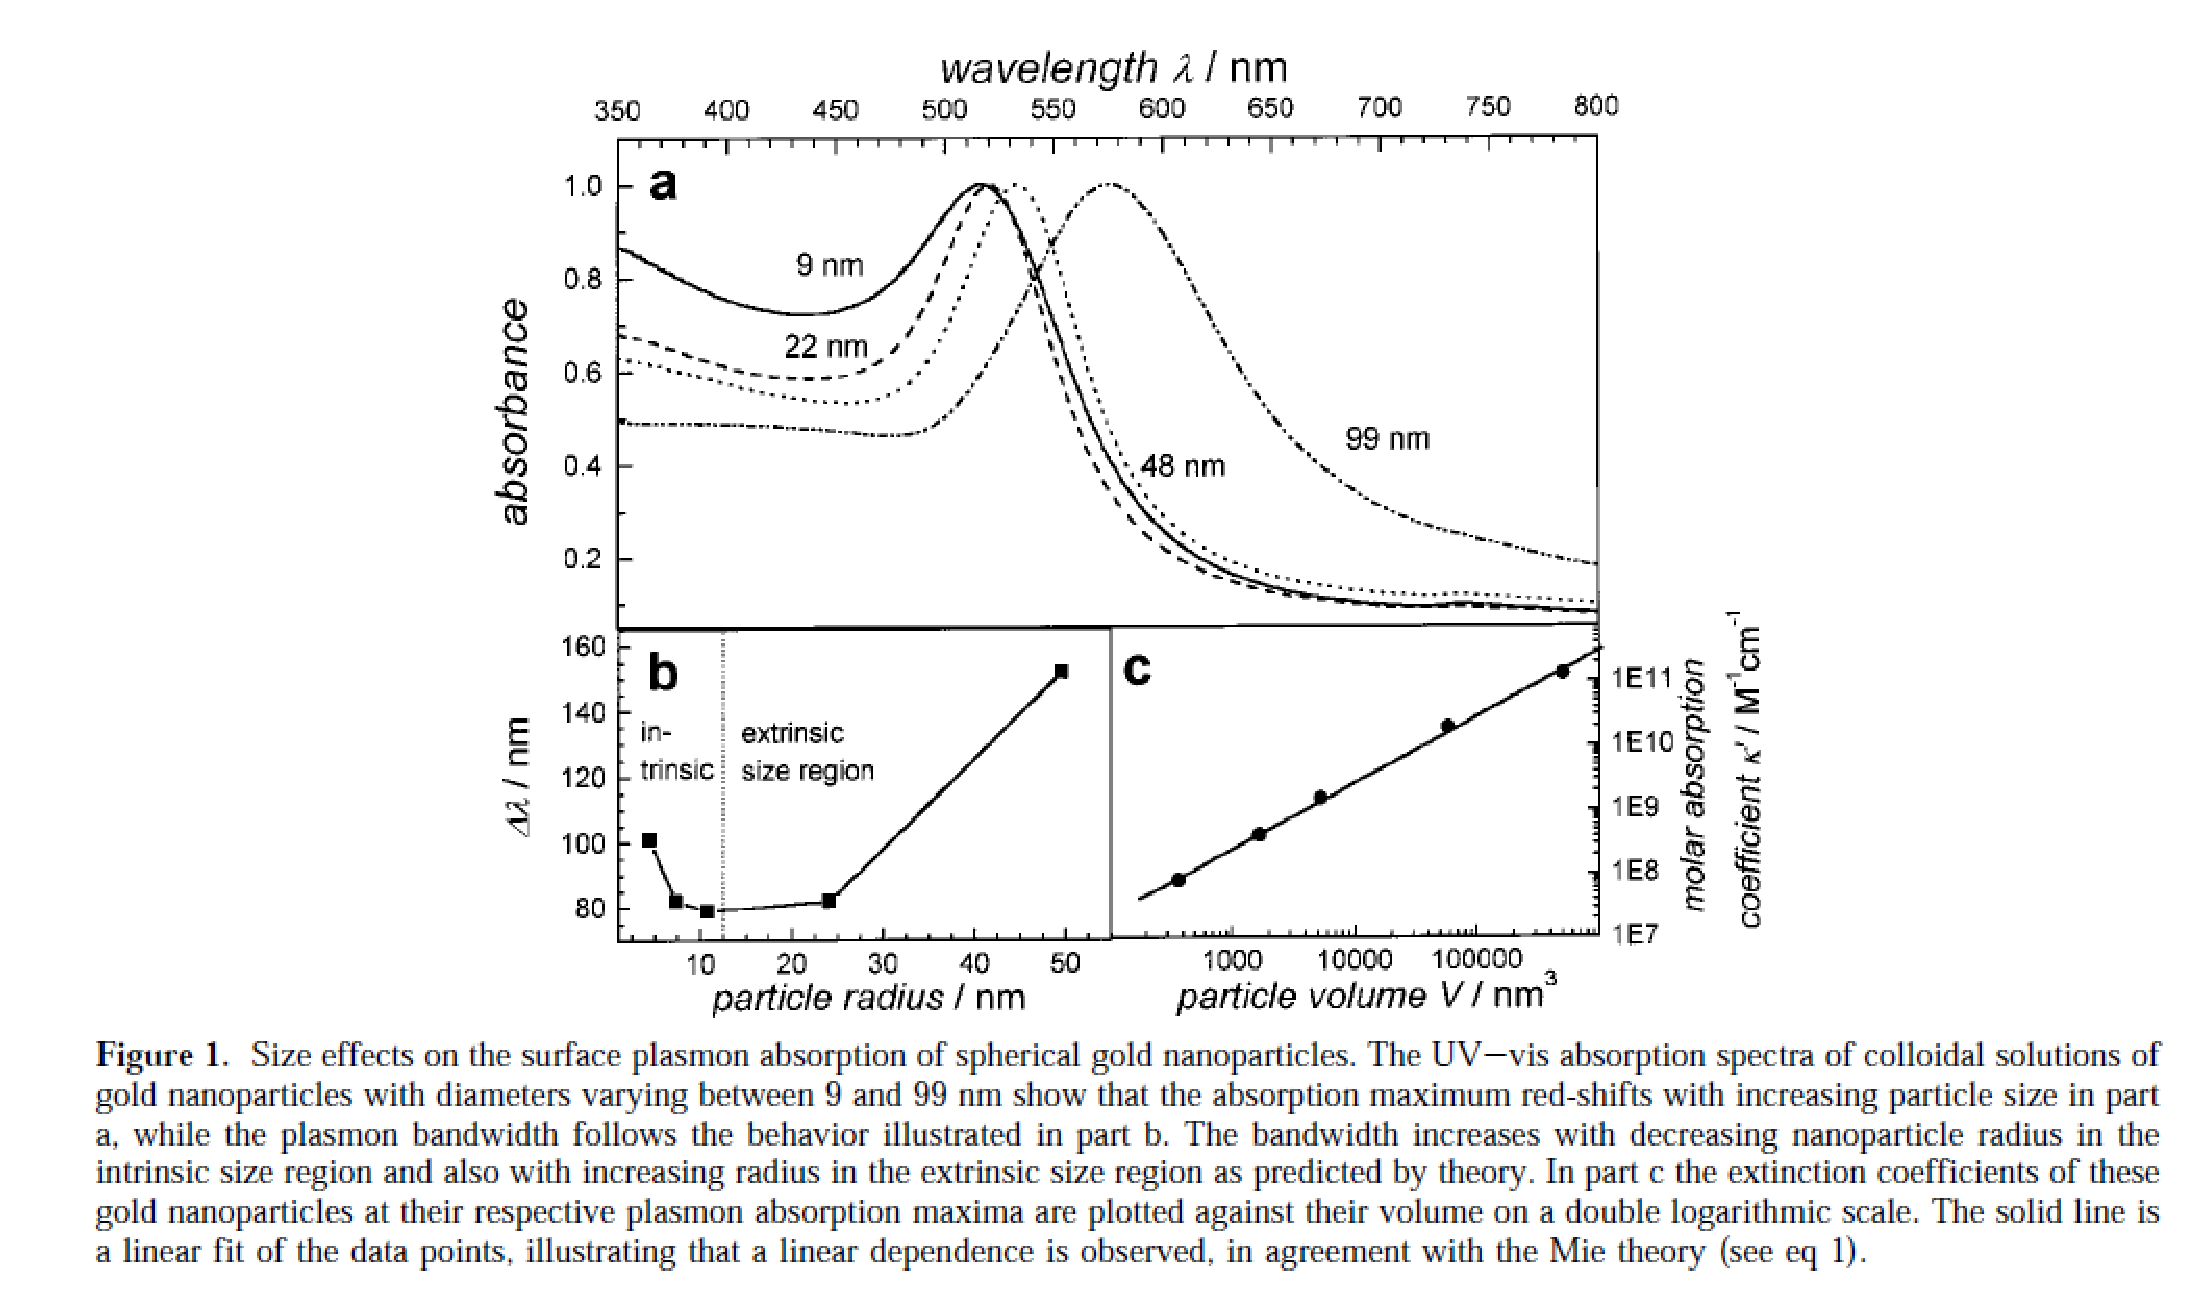
\includegraphics[width=150mm]{images/link99.eps}
		\caption{Measurements of colloidal gold show a peak absorption dependant on size.  A wider distribution of sizes or shapes will produce broadening due to different wavelength centers.  This or another article included a table characterizing shape uniformity which would better illustrate.}
		\label{f:link99}
	\end{figure}
		

	\subsection{How to Evaluate the Reproducibility of Nano-Island Samples}
	The effectiveness of our process control can be evaluated through direct and indirect measurement of the uniformity of the resulting nano-islands.  
	Nano-island size and uniformity can be measured directly through atomic force microscope (AFM) images.  
	Scanning electron microscope (SEM) images may also be used to evaluate size and uniformity, but these images lack resolution to evaluate sizes below {\bf $50nm$ (TBR)}.  
	Spectral measurements of the nano-island samples will show absorption features which can be used, along with the direct measurements, to indirectly indicate the uniformity of the size distribution of the nano-islands.
	
	\begin{quote}
		Because there is inherent heterogeneity among individual nanoparticles, each LSPR spectrum is different, revealing the true distribution of resonance wavelengths (20, 98).		
		\cite{willets2006}
	\end{quote}
	

	\clearpage 
	%% Chapter: Temperature Errors and Controls	%% Chapter: Temperature Errors and Controls	%% Chapter: Temperature Errors and Controls	%% Chapter: Temperature Errors and Controls	%% Chapter: Temperature Errors and Controls	%% Chapter: Temperature Errors and Controls	%% Chapter: Temperature Errors and Controls	%% Chapter: Temperature Errors and Controls
	\section{Temperature Control, Measurement, and Errors}

	In-situ measurements require the measurement of temperature and impedance.  
	The impedance is measured at the sample, while the temperature is inferred from thermocouple measurments.
	Temperature measurments with more than one thermocouple showed that fast heating is uneven across the furnace.  
	Also, during fast heating, impedance measurements of a bare electrode did not match their expected temperature dependance, when the temperature was measured with a nearby 10-mil bare wire K-type thermocouple in air.
	The glass of the electrode caused the sample temperature to lag up to $100^{\circ}C$ behind the air temperature during fast heating.

	\subsection{Temperature Control}

	[ Figures: Furnace Picture, Schematic, McL Engineeing TC shield image ... also link to the Appendix A]

	To allow temperature to be accurately measured (within $50^{\circ}C$ or better) during fast heating, the heating rate must be controlled.
	The COTS Thermolyne furnace temperature controller is a simple PID, which when given a setpoint temperature, will approach this temperature as fast as its capabilities allow.
	To slow the heating to a rate such that the sample temperature may be accurately measured, intermediate PID setpoints must be introduced leading to the final temperature.

	Prior experiments by Toyanath Joshi used a methodical and manual approach of increasing the PID setpoint temperature at the desired rate.
	
	For the research conducted here, an automated PID controller was constructed using Arduino microcontroller, an open-source hardware thermocouple add-on, and the existing solid-state relay within the Thermolyne furnace.  
	The Arduino microcontroller is well-documented (cite:arduino.cc), and its form factor supports a number of add-on boards(``shields'') produced by a large number of independant amateur and commercial vendors.
	The thermocouple ``shield'' contains four addressable MAX31855 thermocouple digitizers with cold-junction compensation and includes connectors for four K-type thermocouples.
	The solid-state relay within the Thermolyne furnace was easy to control, as the old PID control could be simply disconnected and swapped for a new controller (include pic when i'm willing to do disconnect the furnace).

	The Arduino has a USB computer interface but also runs stand-alone code independantly of the computer.
	This means the oven temperature is always controlled by the microcontroller, but the computer interface may be used to request changes to the program running on the controller.
	The computer is used to set a final setpoint temperature and a rate at which the temperature should be approached.  
	The microcontroller uses these two parameters, along with the current temperature measured from its sensor, to break the ramp into a time-dependant setpoint temperature to pass to a PID algorithm.
	The PID algorithm decides how best to approach the current setpoint (which will change over time), and over time, the fial setpoint will be reached.

	[the PID is better described by code or flow chart than equation]


	In the modified temperature controller, any single one of four thermocouples can be used in the PID controller.	
	
	

	\subsection{Temperature Measurement}
	
	\begin{figure}
		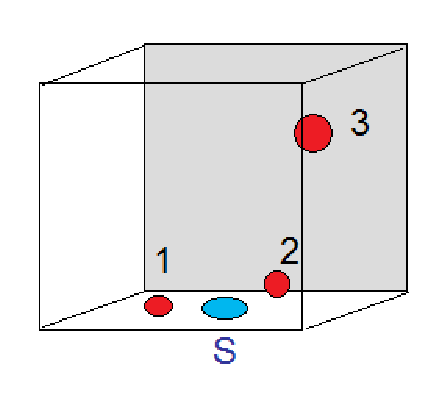
\includegraphics[width=70mm]{images/oven_tc_placement.eps}
		\caption{Placement of the three thermocouples and the sample within the furnace used to measure furnace/sample temperature.  TC1 is the glass-slide thermocouple, TC2 is a bare TC, TC3 is the furnace TC, and S is the sample.}
		\label{f:furnace_tc}
	\end{figure}
	
	\begin{figure}
		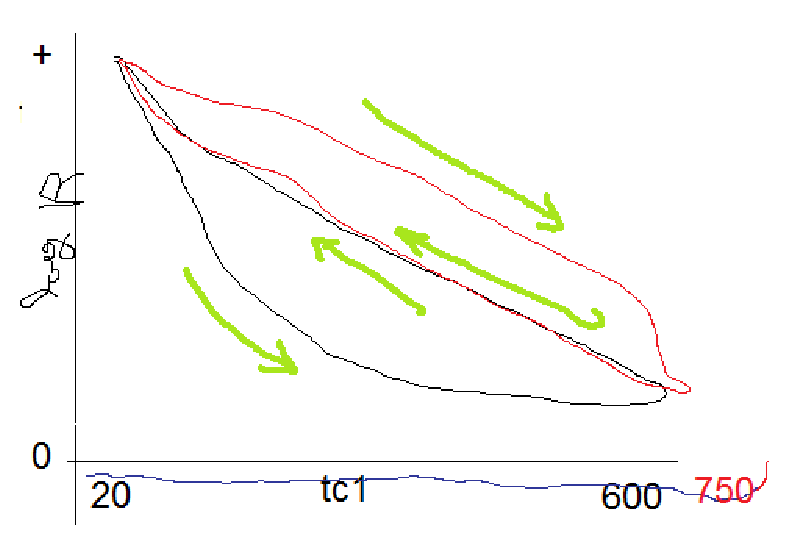
\includegraphics[width=150mm]{images/plot_logR_vs_tc1_and_tc3.eps}
		\caption{If temperature is accurately measured, the log impedance of the bare IDE sample will match on heating and cooling.  If the thermocouple temperature heats faster than the sample, the sample resistance will appear higher on (fast) heating than (slow) cool-down (red trace).  If the thermocouple temperature lags the sample temperature on heating, the sample resistance will appear lower on heating than cool-down (black trace).  The closer the overlap between heating and cooling, the better the thermocouple matches the temperature seen by the sample. }
		\label{f:logR_vs_t1_and_t3}
	\end{figure}
	
	\begin{figure}
		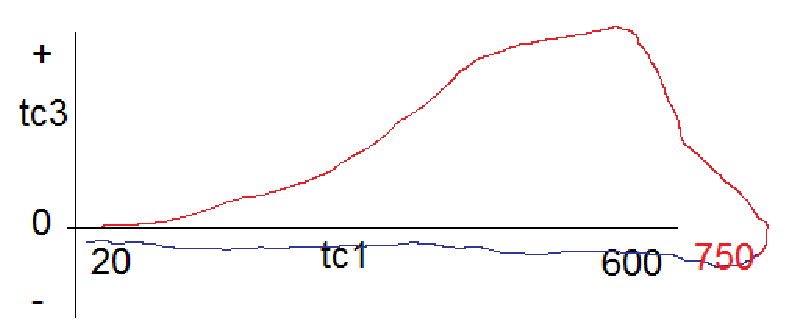
\includegraphics[width=150mm]{images/residual_plot_tc3_vs_tc1.eps}
		\caption{f:plot\_tc3\_vs\_tc1}
		\label{f:plot_tc3_vs_tc1}
	\end{figure}
	
	Use of multiple thermocouples (Figure ~\ref{f:furnace_tc}) to measure furnace temperature during very rapid heating showed large temperature gradients within the furnace, and that the glass slides on which the samples are mounted slow the heating of the sample.

	Three thermocouples were used to measure furnace temperature.  
	The furnace has a heavy gauge K-type thermocouple at the top of the furnace (tc3 in Figure ~\ref{f:furnace_tc}).  
	A bare 10 mil ($254{\mu}m$) thermocouple (tc2 in Figure ~\ref{f:furnace_tc}) was situated near the bottom of the furnace.  
	A third thermocouple (tc1 in Figure ~\ref{f:furnace_tc}) was attached to a glass microscope slide with a dab of silver epoxy and placed next to the sample.
	
	The IDE sample is responsive to temperature, and a bare IDE should show the same impedance during (fast) heating as it shows during (slow) cooling (Figure ~\ref{f:logR_vs_t1_and_t3}).  
	If the temperature measured by a thermocouple results poor overlap of the IDE impedance on the heating and cooling phases, a temperature error can be inferred.
	In this way the bare slide can serve as a fourth temperature-sensitive device to confirm that the "sample temperature" inferred from the thermocouple temperature measurements accurately tracks temperature.  
	
	The furnace PID controller creates a closed-loop temperature control system, using a single thermocouple to measure the furnace temperature, and a solid-state relay to turn the furnace on and off. 

	In the modified temperature controller, any thermocouple can be used in the PID controller.	
	
	For all furnace tests in Spring 2012, we selected a thermocouple mounted to a glass slide by silver epoxy to close the loop of the PID system.
	Since the glass-slide TC best tracks the temperature of the IDE sample, it was believed to result in fastest heating.
	However, because the glass is slower to heat than the air, it can cause a situation in which the furnace overheats. 
	
	It was discovered in early testing that the glass slide IDE lags behind the temperature at the top of the furnace by as much as $200^{\circ}C$ during fast heating of $30^{\circ}C/min$ (Figure ~\ref{f:residual_plot_tc3_vs_tc1}).  
	The build-up of heat and the lag of the glass TC resulted in an overheating of the oven when there is no additional safety measures.  
	A safety measure was introduced into the furnace controller code to turn off the heat if any TC measured greater than $+50^{\circ}C$ from the furnace setpoint.

	For all furnace tests in Summer 2012, we selected a bare thermocouple positioned at the bottom of the furnace (tc2 in Figure ~\ref{furnace_tc}) to close the loop of the PID system.
	Use of the bare TC in the PID system avoids the problem of overheating, and in testing (Section ~\ref{sec:Temperature_Uniformity_Three_Slides}), the glass slide temperature was controlled under fast heating to $625^{\circ}C$ at a rate of $30^{\circ}C/min$ with an overshoot of the sample temperature (measured by the glass slide) of just $2^{\circ}C$  [TBR].  
	The lack of run-away heating results from the rapid response of the glass slide thermocouple to small changes in air temperature within the furnace, and the mass of the glass slide which causes a slow approach to the final temperature.

	
	\subsection{Temperature Errors: Fast Heating is Uneven} \label{sec:Temperature_Uniformity_Three_Slides}

	\subsubsection{Analysis of Furnace Temperature Uniformity Using Three Glass Slide Thermocouples}

	\begin{figure}
		\includegraphics[width=140mm]{images/Oven_Thermocouple_4x.eps}
		\caption{Additional glass slide thermocouples were produced and used to measure the uniformity of the furnace temperature and similarity among glass-slide thermocouples.  Three glass slide thermocouples were used for measurement, and a fourth bare TC was used in the PID controller during this test.}
	\end{figure}
	\begin{figure}
		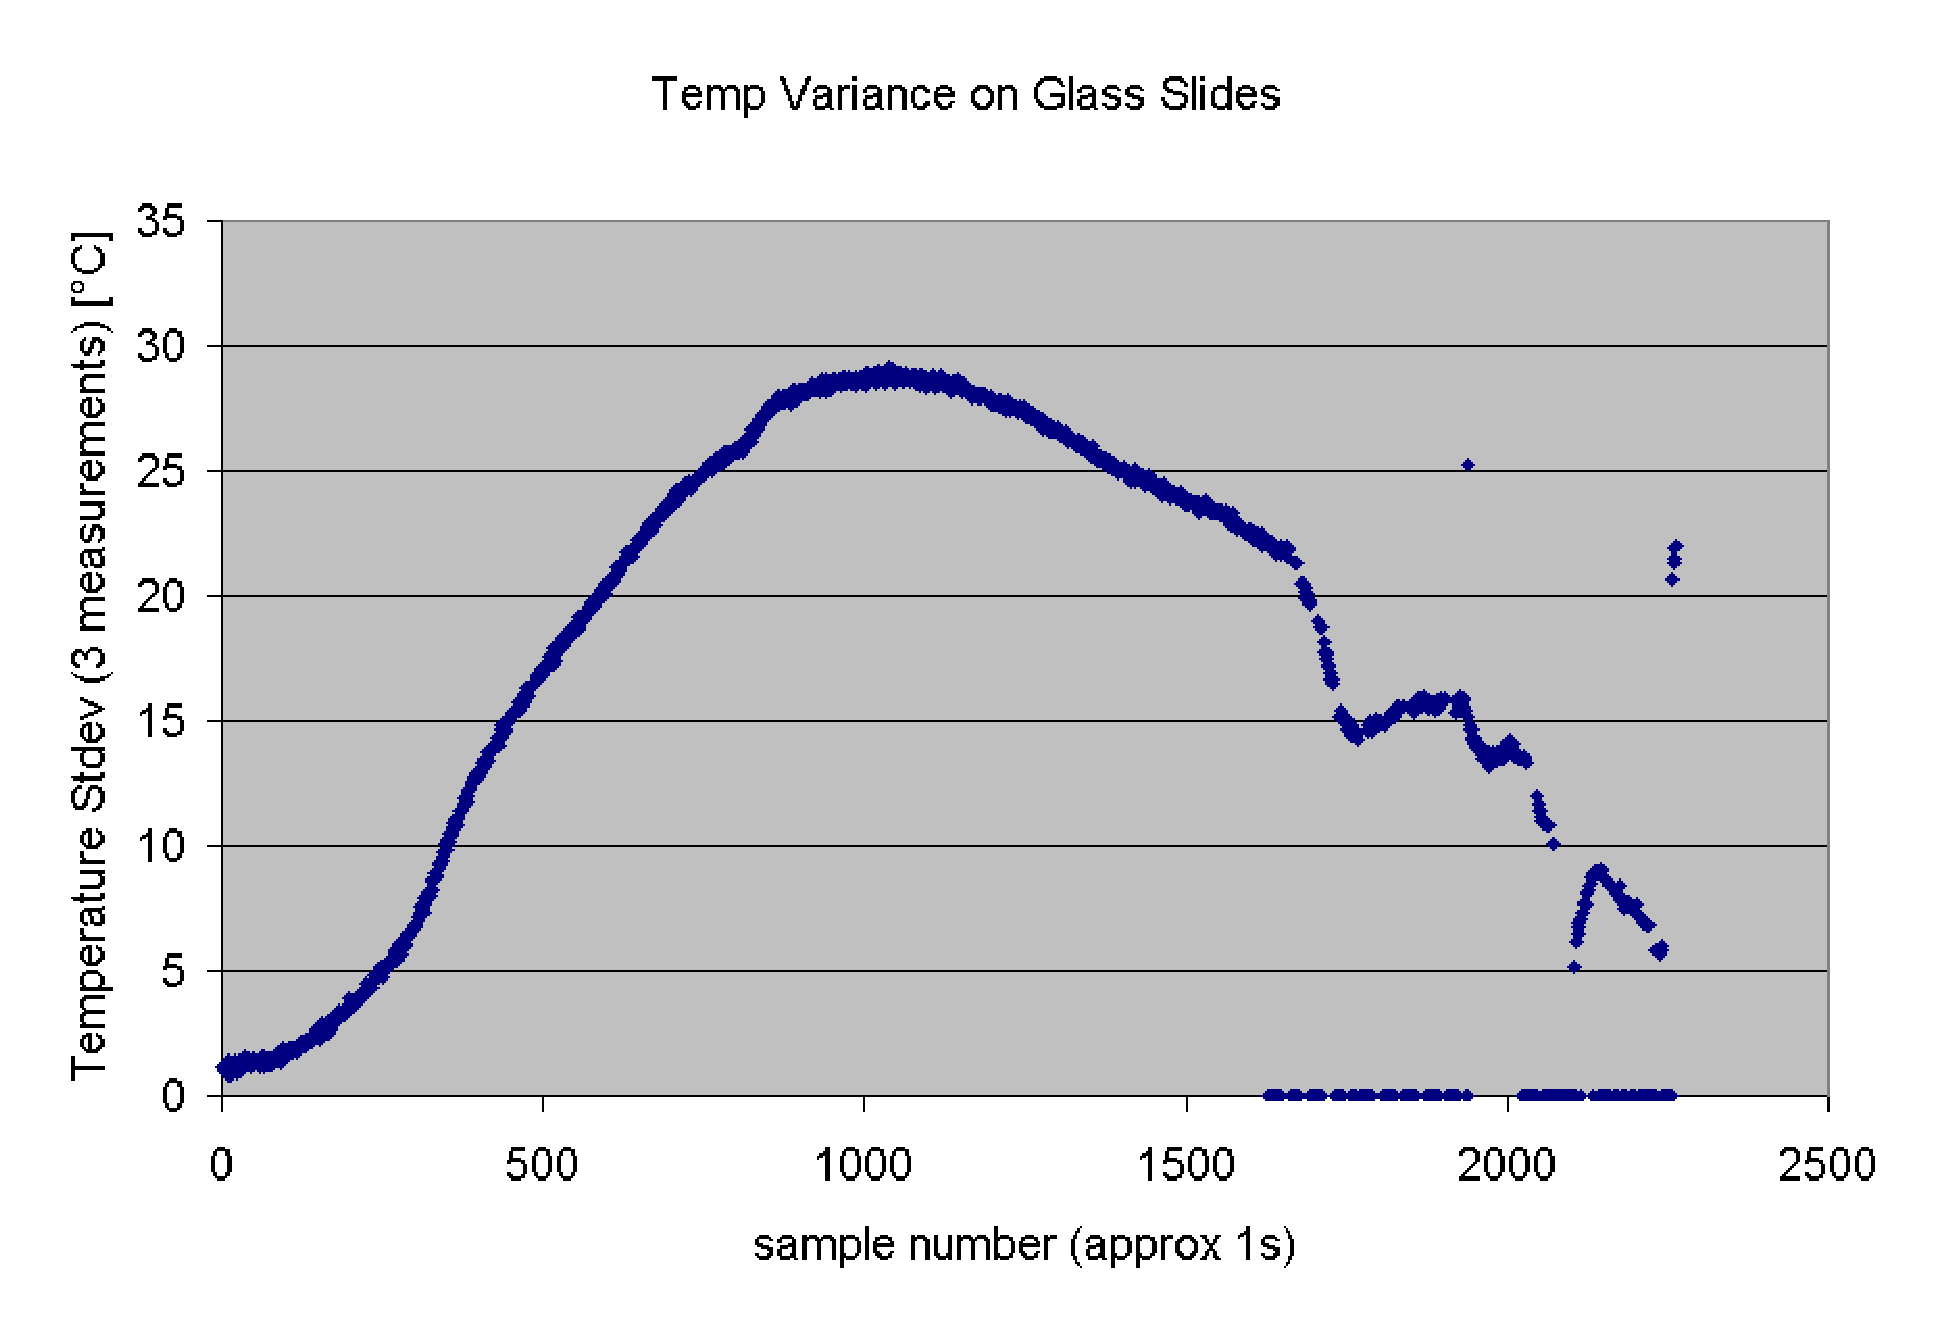
\includegraphics[width=140mm]{images/heating_data.eps}
		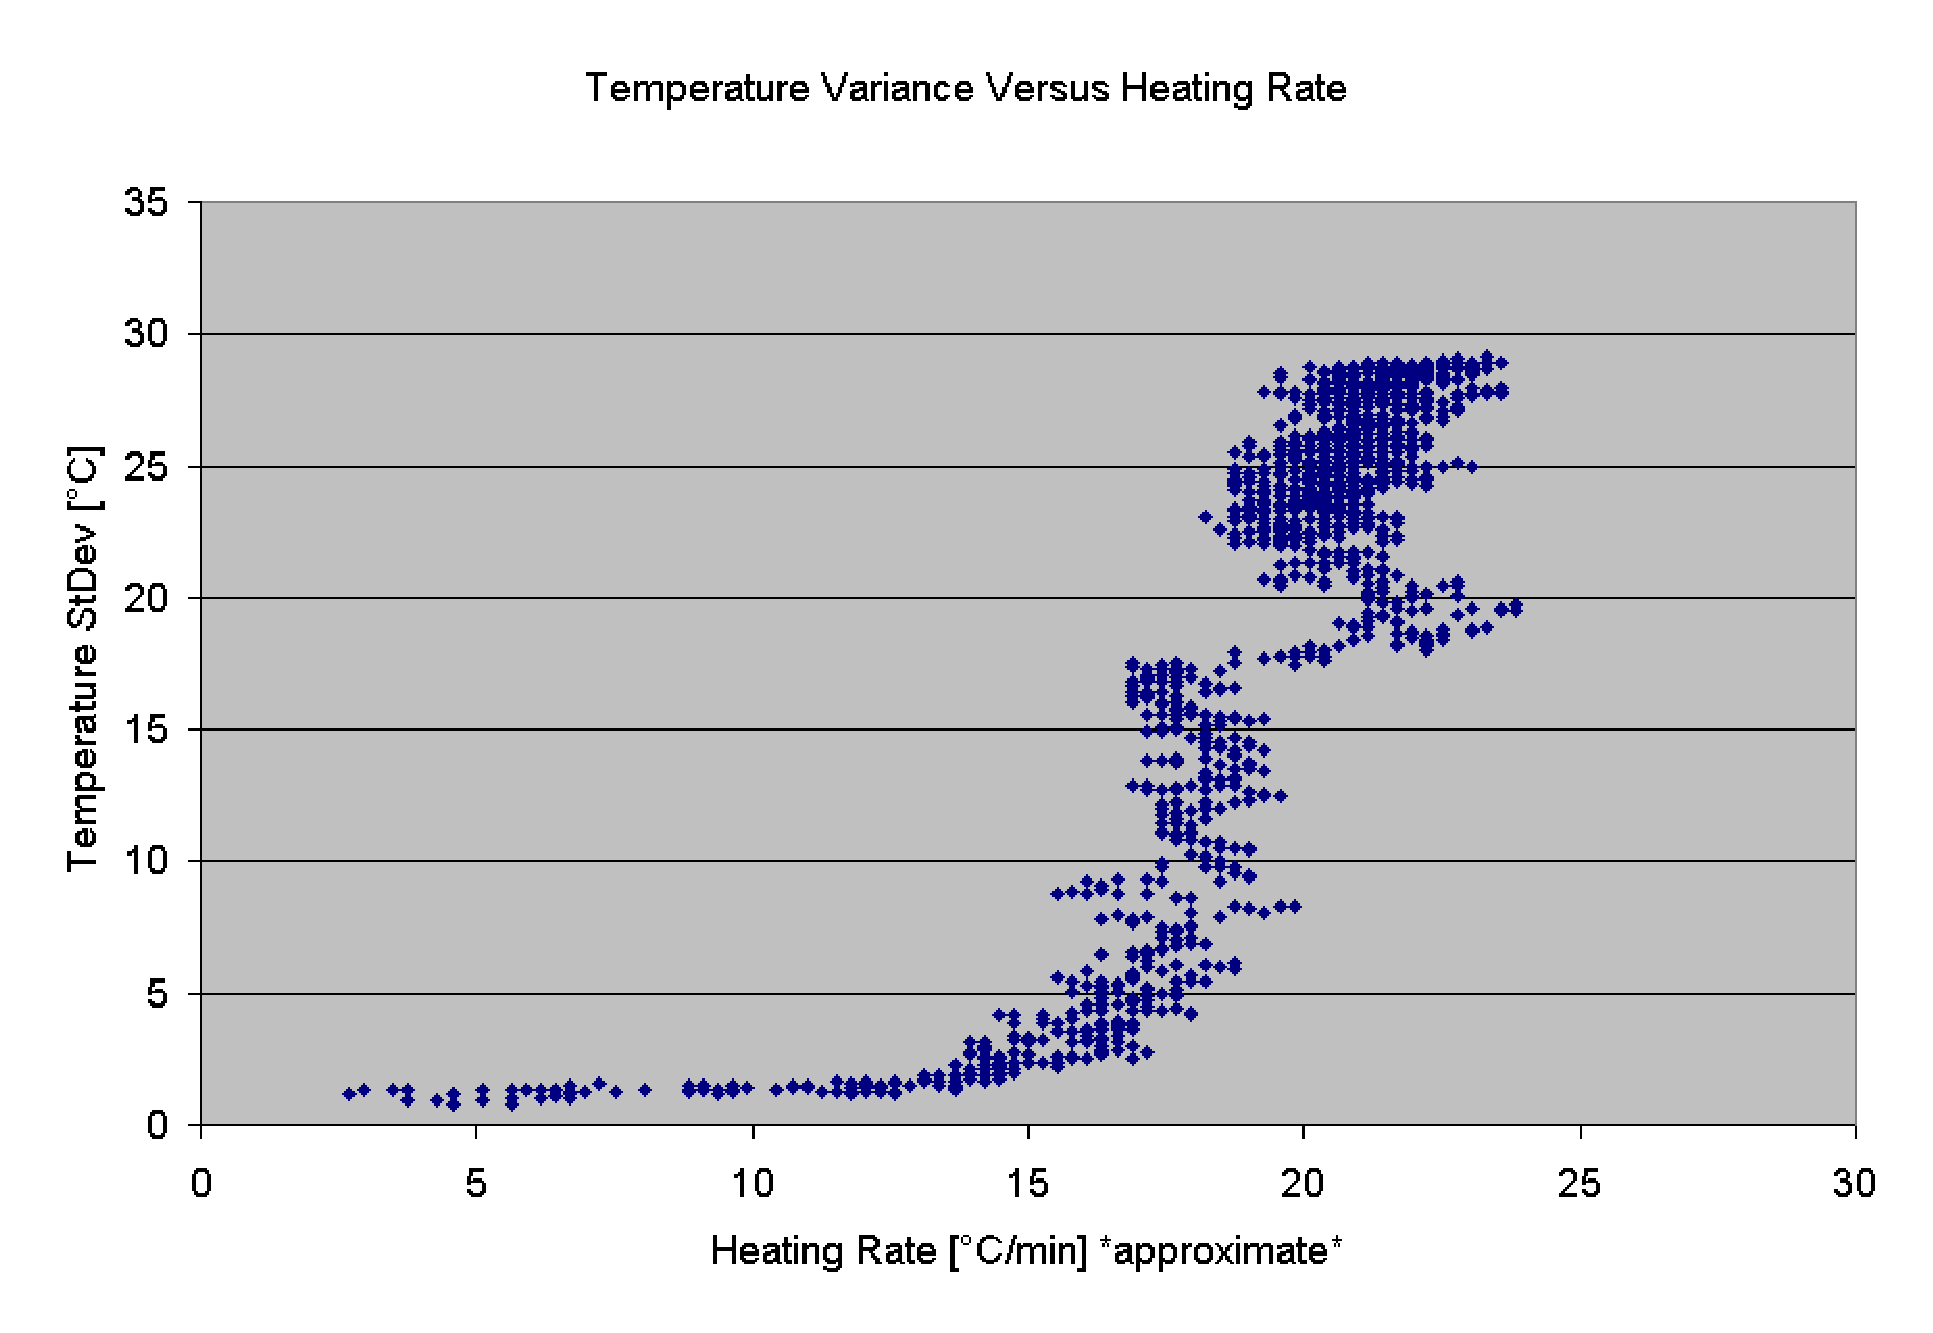
\includegraphics[width=140mm]{images/variance_vs_rate.eps}
		\caption{The plot at left shows the standard deviation among the three glass slide thermocouples during fast heating, which is approximately the magnitude of the bias uncertainty in temperature during heating.  The temperature variance versus heating rate is plotted at left.  The magnitude of the temperature gradients across the base of the furnace are non-linearly proportional to temperature.}
	\end{figure}
	
	To test the reproducibility of the glass slide thermocouple, three glass slide thermocouples were made, by affixing a K-type thermocouple to the surface of a glass microscope slide.
	A fourth thermocouple was left bare and placed at the bottom of the furnace for use in the PID temperature controller.
	While the glass slide thermocouple can be used in the PID loop to raise the furnace temperature, it requires a gradient limiter to function safely.  
	The gradient limiter shuts off heating if the temperature between any two thermocouples exceeds a threshold ($50^{\circ}C$ was used), and is best used with one thermocouple at the top of the furnace (otherwise the gradient is not well sampled).

	Because the temperature controller built for this project is limited to four K-type thermocouples, a trade-off was made between fast heating (for which a glass slide TC is used) and complexity (the requirement that the heating gradient be limited). 
	A consequence to using an furnace shut-off is that the heating is no longer at an even rate, and the temperature characterization emphasizes errors (Figure "shutoff emphasizes errors in Au25 test").

	Results of the glass slide thermocouple uniformity measurement shows that three glass slides placed across the bottom of the furnace, when heated at a rate $25^{\/circ}C$ per second, show a disagreement of $X^{\circ}C$ at the fastest rate of heating (Figure "three slides result").

	\clearpage
	
	\section{In-Situ Transport Measurements and Complex Impedance}

	\subsection{Electron Transport Measurement using Complex Impedance}
	A four-point impedance measurement measures complex impedance of the IDE sample under test (device under test, or DUT).  
	Impedance measurements follow a temperature dependence derived from models of electron transport under an AC potential.  
	Complex impedance and temperature measurements are used to solve electron mobility under the AC electron transport model detailed below.  
	Temperature measurements were limited to those measurements taken during cool-down of the DUT, since temperature measurements during fast heating of the sample carry very large errors.  
	Measurements of impedance over temperature during cool-down (FIGURE "cooldown\_residuals") were identical within uncertainties for the Au$_25$ sample (JD04) and a bare IDE sample (JD05), and electron mobility will be identical.  
	Electron mobility calculated for the Au$_25$ (JD04) sample was ${\epsilon\over{k}} = 1.1e+04 K$, $\epsilon = 0.96 eV$.
		
	\subsubsection{Introduction: Measurement of Complex Impedance} 
	DC resistance measurements of the electrode show only its insulating properties, as the glass substrate is a poor conductor and the IDE is a weak capacitor, so AC resistance is measured.
	AC resistance in the IDE samples follows the temperature-dependent electron mobility.
	
	\begin{equation}
		R = R_0 \cdot e^{\epsilon\over{k \cdot T}}
		\label{eq:emobility}
	\end{equation}
	
	This equation can be rearranged into a linear equation to solve for $\epsilon$.
	
	\begin{equation}
		ln(R) = {\epsilon\over{k}} {1\over{T}} - ln(R_0)
		\label{eq:solve_emobility}
	\end{equation}
	
	${\epsilon\over{k}}$ and $ln(R_0$ are found by least-squared fit of the linear portion of the data.
	
	\begin{figure}
	
	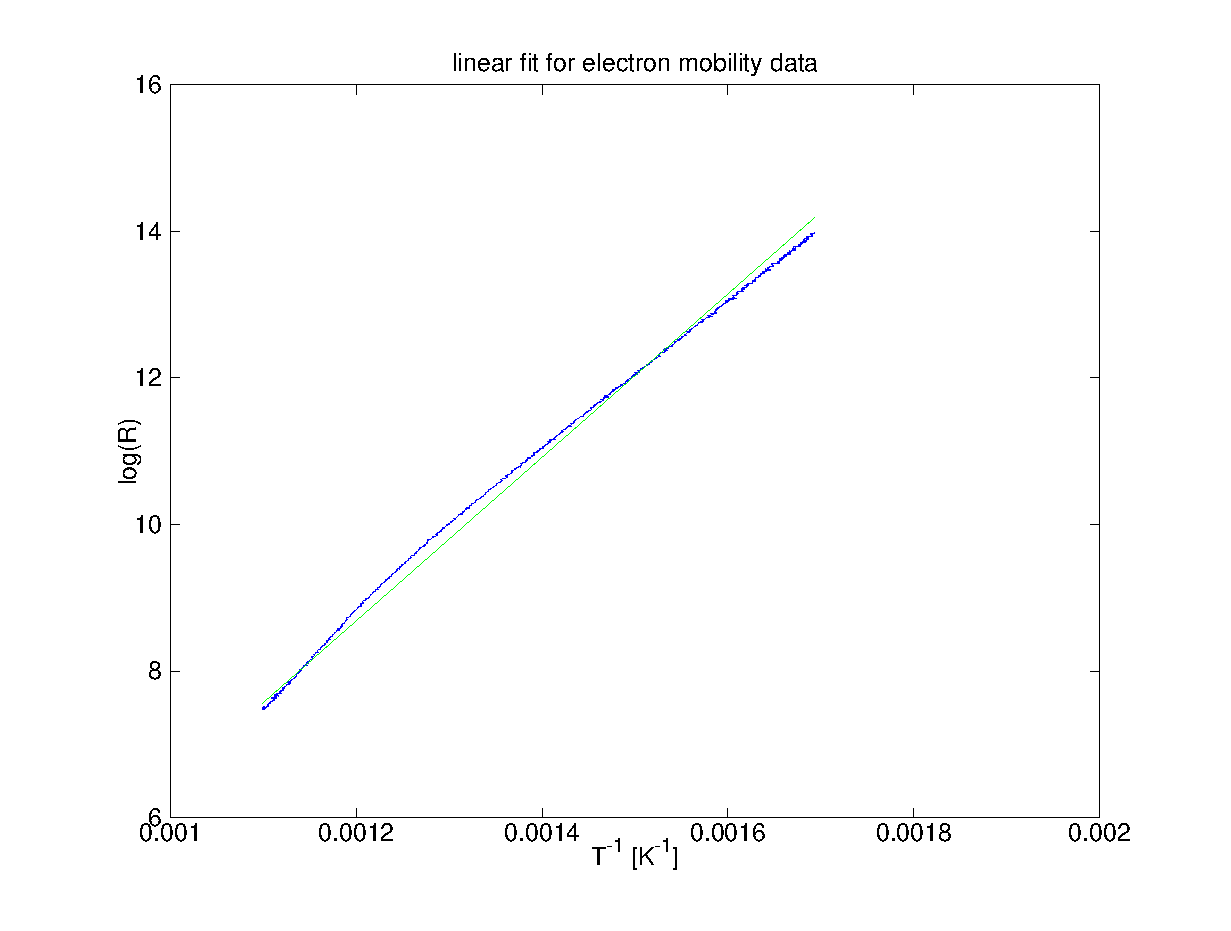
\includegraphics[scale=0.4]{images/electron_mobility.eps} 
	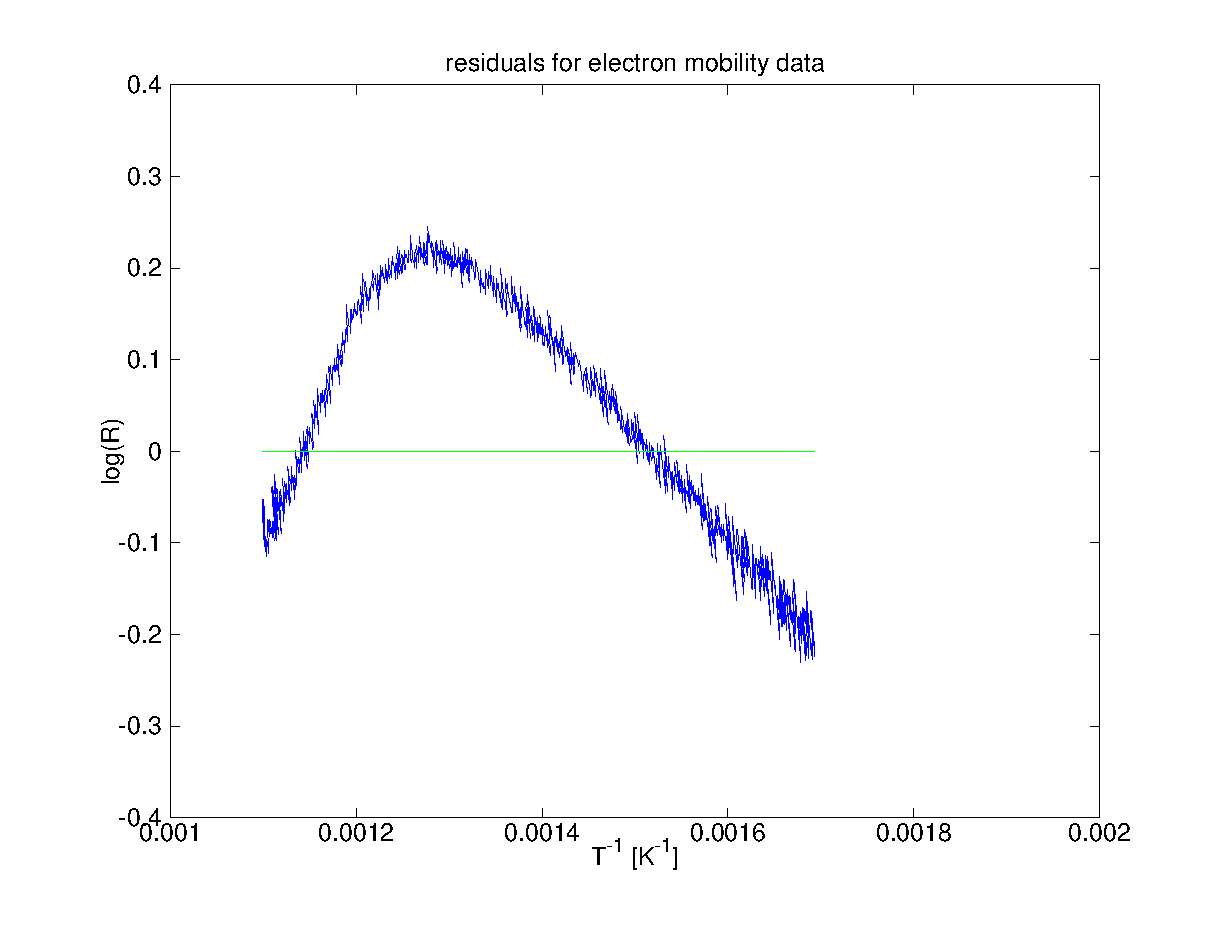
\includegraphics[scale=0.4]{images/electron_mobility_residual.eps}
	\label{f:emobility}
	\caption{During cool-down of the sample, the impedance versus temperature measurements are well-sampled, and can be used to solve for electron mobility.  ${\epsilon\over{k}} = 1.1e+04 K$, $\epsilon = 0.96 eV$, $R_0 = 9.1e-3\Omega$.  Error bars are needed, and will have magnitude at least proportional to the fit residuals.}
	\end{figure}
	The temperature range observed is between $295K$ and $900K$, 
	
	Sample resistance (a parallel AC resistance) is typically high for the sample under test, this resistance changes when the sample is heated and the polymers are burned off.  

	The resistance $R_p$ of a high-resistance sample can be measured from the complex impedance $(Z,\theta)$ by Equation ~\ref{eq:R_p}.  Use of the parallel resistance $R_p$ is justified at high sample resistance because the series resistance $R_s$ of the test leads and contacts are orders of magnitude smaller.
	
	\begin{equation}
		R_p = {{Z} \over {cos({\theta})}}
		\label{eq:R_p}
	\end{equation}
	
	Typical values for complex impedance measured by the auto-balancing bridge method via an Agilent 82XX LCR meter are as follows.
	
	\begin{equation}
		\left( Z,\theta,\nu,T \right) = \left( 15 M\Omega, -89.9^\circ, 1kHz, 22^{\circ}C \right)
	\end{equation}
	\begin{equation}
		\left( Z, \theta, \nu, T \right) = \left( 800 k\Omega, -88^\circ, 45kHz, 22^{\circ}C \right)
	\end{equation}
	
	This result shows that the $R_p$ ``resistance'' component (which is $Z$ divided by $cos(-89^\circ)$) is immeasurably high at low frequencies and low temperature.  It is only at higher temperatures that $R_p$ drops to the measurable range, and this occurs at about $250^{\circ}C$ when the impedance phase angle $\theta$ drops from $-89.9^\circ$ towards $0.1^\circ$.
	
	During the burn-off of the polymers, the parallel resistance may drop to under 100 ohms, which requires a four-point measurement to compensate for the series resistance test lead impedance.
	A four-point measurement is necessary because the test leads have been reported (AD5933) to have up to kilo-ohm impedance when measuring low sample resistance.


	\section{ Post-Processing Measurement Methods Discussion }
	\subsection{AFM}
	\subsection{SEM}
	\subsection{LSPR}



	\section{Gold Nano Island Preparation}	

	\subsection{Preparing Gold Slides}
	
	\subsubsection{Preparation of Gold Nanoparticle Solution}
	The preparation of the gold nanoparticle solution requires about a week of preparation to yield the 10 mL of Au$_{314}$.
	

	\subsubsection{Layering the Samples}
	To deposit the self-assembling multilayers on a glass electrode, the following steps are 
	\begin{itemize}
		\item First Day
		\begin{itemize}
			\item An aqueous solution of poly(allylamine hydrochloride) (PAH) is prepared, adding 10mg PAH to 10mL nanopure water, for use on Day Three.
			\item 1.0mL methanol is added to 0.1mL triethyl 3-mercaptopropylsilane in a 5mL vial.
			\item 0.1mL of nanopure water is added to the solution.  (The triethyl 3-mercaptopropylsilane will react with the water and the solution becomes cloudy).
			
			\item The IDE is placed in the solution for 24 hours.
			\item \emph{Note}: it is important not to leave the IDE for more than 24 hours, or the IDE will acquire a thick deposited coating.
		\end{itemize}
		\item Second Day
		\begin{itemize}
			\item The IDEs are placed in clean 5mL vials.
			\item Methanol is added to the vials and the samples are sonicated in an ultrasonic bath.
			\item The methanol wash is removed, and the washing process is repeated 2 more times.
			\item After the third ultrasonic wash, the samples are gently dried under a stream of nitrogen gas or air.
			\item After drying, gold nanoparticle solution is added to each vials, enough to cover the IDE.
			\item The IDEs are left in the nanoparticle solution overnight.
		\end{itemize}
		\item Third Day
		\begin{itemize}
			\item A work station is prepared with an ultrasonic bath, Pasteur pipettes, nanopure water, ethanol, PAH solution, and several spare 20mL vials for containing waste or re-used liquids.
			\item for layer = 2:10 
			\begin{itemize}
				\item The gold nanoparticle solution is removed from each vial using Pipette A and placed in a 20mL vial for reuse.
				\item A washing solution of nanopure water (Au$_{25}$) or ethanol (Au$_{314}$) is added to each vial using Pipette A, and the vials are placed in an ultrasonic bath.
					\subitem Washing the IDE by inverting the vials is not recommended, as this breaks bonding wires.  An ultrasonic bath prevents damage to the wire bonds.
				\item If the nanoparticle solution is Au$_{314}$, the ethanol is removed with Pipette A, nanopure water added, and the vials are again placed in the ultrasonic bath.
				\item The nanopure water is removed from the vial (for Au$_{314}$ and Au$_{25}$) using Pipette A.
				\item The PAH solution is added to each vial using Pipette B and the vials are left to stand for 5 minutes.
				\item The PAH solution is removed from the vials using Pipette B,  nanopure water is added with Pipette B, the vials are placed in an ultrasonic bath, and the nanopure water is removed using Pipette B.
				\item If Au$_{314}$, then add ethanol using Pipette A and place the vial once more into the ultrasonic bath, and the ethanol is removed with Pipette A.
				\item If this layer is not the last layer, the Au$_{314}$ or Au$_{25}$) solution is added to the vials using Pipette A, and the vials are left to stand for 5 minutes.
			\end{itemize}
			\item end for loop (next layer)
			\item The IDEs are gently dried under a stream of nitrogen gas or air, and placed in a vacuum desiccator in the dark, for storage.
		\end{itemize}
	\end{itemize}

	\subsection{Bonding and Baking}
	
	\subsubsection{Attaching Bonding Wires for Four-Point Impedance Measurement}
	[ Discussion and images of two methods of bonding used in this study ]
	
	
	\section{Electron Transport Measurements of Au$_{25}$}
	\subsection{Setup/Procedure}
	\subsection{Impedance, Temperature Measurements, AFM/SEM Images, LSPR}
	\subsection{Conclusions}

	\section{Electron Transport Measurements of Au$_{314}$}
	\subsection{Setup/Procedure}
	\subsection{Impedance, Temperature Measurements, AFM/SEM Images, LSPR}
	\subsection{Conclusions}




\clearpage
\bibliography{thesis_draft}
\bibliographystyle{plain}


\end{document}

%% ******************************************************************
%% The following is some template materials -- equations and figures.
\documentclass[aps,prl,twocolumn,oneside,showkeys,floatfix]{revtex4-1}
\newcommand{\BibTeX}{{\sc Bib}\TeX}
\usepackage{graphicx}
\usepackage{listings}

\newbox\bwk\edef\tempd#1pt{#1\string p\string t}\tempd\def\nbextr#1pt{#1}
\def\npts#1{\expandafter\nbextr\the#1\space}
\def\ttwplink#1#2{\special{ps:1 0 0 setrgbcolor}#2\special{ps:0 0 0 setrgbcolor}\setbox\bwk=\hbox{#2}\special{ps:( linkto #1)\space\npts{\wd\bwk} \npts{\dp\bwk} -\npts{\ht\bwk} true\space Cpos}}
        \begin{equation}
        \nu_{\mathtt{Larmor}} = {{\Delta E} \over{ 2 \pi \hbar}} = {{2 B \cdot \mu_{\mathtt{proton}}} \over{2 \pi \hbar}}
        \end{equation}

        \author{John \surname{Donovan}}
        \affiliation{CSULB}
        \begin{abstract}
                \begin{description}
                        \item[Background] This part would describe the
                        context needed to understand what the paper
                        is about.
                        \item[Purpose] This part would state the purpose
                        of the present paper.
                        \item[Method] This part describe the methods
                        used in the paper.
                        \item[Results] This part would summarize the
                        results.
                        \item[Conclusions] This part would state the
                        conclusions of the paper.
                \end{description}
        \end{abstract}
        \keywords{nano,nano-islands,thin films}
        \maketitle
        Written in \LaTeX\ with TexMaker.


\begin{figure}
\includegraphics[scale=0.5]{BField_Set1.eps} \label{BSet1}
\caption{The magnetic field (in MHz resonance frequency) measured.  Set 1 did not include many measurements of the most uniform part of the field.}
\end{figure}

\clearpage
\begin{widetext}
\section{Appendix}
\subsection{Spin Echo Peak-Finder Algorithm in Matlab}
\lstset{language=Matlab, basicstyle=\footnotesize, numbers=left, captionpos=t, breaklines=true, caption=find\_spin\_echo() locates the pulse maxima in a spin-echo pulse train, label=T2 Pulse Train, frame=shadowbox}
\lstset{basicstyle=\small\ttfamily, basewidth=0.51em}
\lstinputlisting{../find\_pulse\_train.m}
\end{widetext}

%% *******  END OF TEMPLATE MATERIALS  ******************************
%% ******************************************************************

%% *******  Draft Material *******
